\textbf{Thesis Statement:} I propose a novel, neural-based mention-pair model for cross-document coreference resolution for events, which uses few lexical features and addresses shortcomings of traditional clustering approaches.  I will extend this work by jointly modelling both entities and events, while using structured information (e.g, parse trees).  Last, we aim to improve mention detection, whereby we develop an all-inclusive, end-to-end system which jointly resolves mention boundaries and coreference predictions.

\vspace{10mm}

% ====================
\section{Motivation}
% ====================
Coreference Resolution remains a fundamental NLP task, as it is an essential component for any system that desires ``understanding'' textual data.  That is, in order to accurately model meaning, one must at the very least understand which items are concerning the same underlying objects.  As a simple example, if one performs a Web search for ``President Barack Obama'', some of the web page search results will contain sentences which only refer to him as ``Obama'', ``he'', or "The President," and correctly using this information is essential for returning relevant information to the user's query.  Further, coreference resolution is useful for information extraction \cite{Humphreys:1997:ECI:1598819.1598830}, question answering \cite{Narayanan:2004:QAB:1220355.1220455}, topic detection \cite{Allan:1998}, summarization \cite{Daniel:2003}, and more.

% ====================
\section{Problem Statement}
% ====================
Coreference resolution is the task of identifying -- within a single text or across multiple documents -- which \textit{mentions} refer to the same underlying discourse object. 

A \textbf{mention} is a particular instance of word(s) in a document which represent an \textit{entity} or \textit{event}, such as \textit{Barack Obama}, \textit{he}, or \textit{announced}.

An \textbf{entity} may be a person, location, time, or an organization.  The mentions which refer to them may be \textit{named}, \textit{nominal}, or \textit{pronominal}:
\begin{itemize}
\item Named mentions are represented by proper names (e.g., Andr\'e Benjamin or Pakse, Laos) 
\item Pronominal mentions are represented by pronouns (e.g., she or it)
\item Nominal mentions are represented by descriptive words, not composed entirely of a named entity or pronouns (e.g., The well-spoken citizen)
\end{itemize}

An \textbf{event} can generally be thought of as a specific action.  Quine \cite{quine1985} was the first to propose that an event refers to a physical object which is grounded to a specific time and location, and that two events are identical (i.e., co-referent) if they share the same spatiotemporal location.  This definition has become the general consensus within the community\footnote{Hovy, et. al. \cite{Hovy2013EventsAN} provide an in-depth study of varying definitions.}.  Specifically, two co-referent events must share the same \textit{properties} and \textit{participants}.  For example, in Figure \ref{fig:corpus}, sentences \#1 and \#2 contain the co-referent events (``placed'' and ``put''), yet neither are co-referent with events in sentence \#3.  Often times, the participants (arguments) may be referred to in different ways, implied, or missing altogether.

\begin{figure}[ht]
\centering
	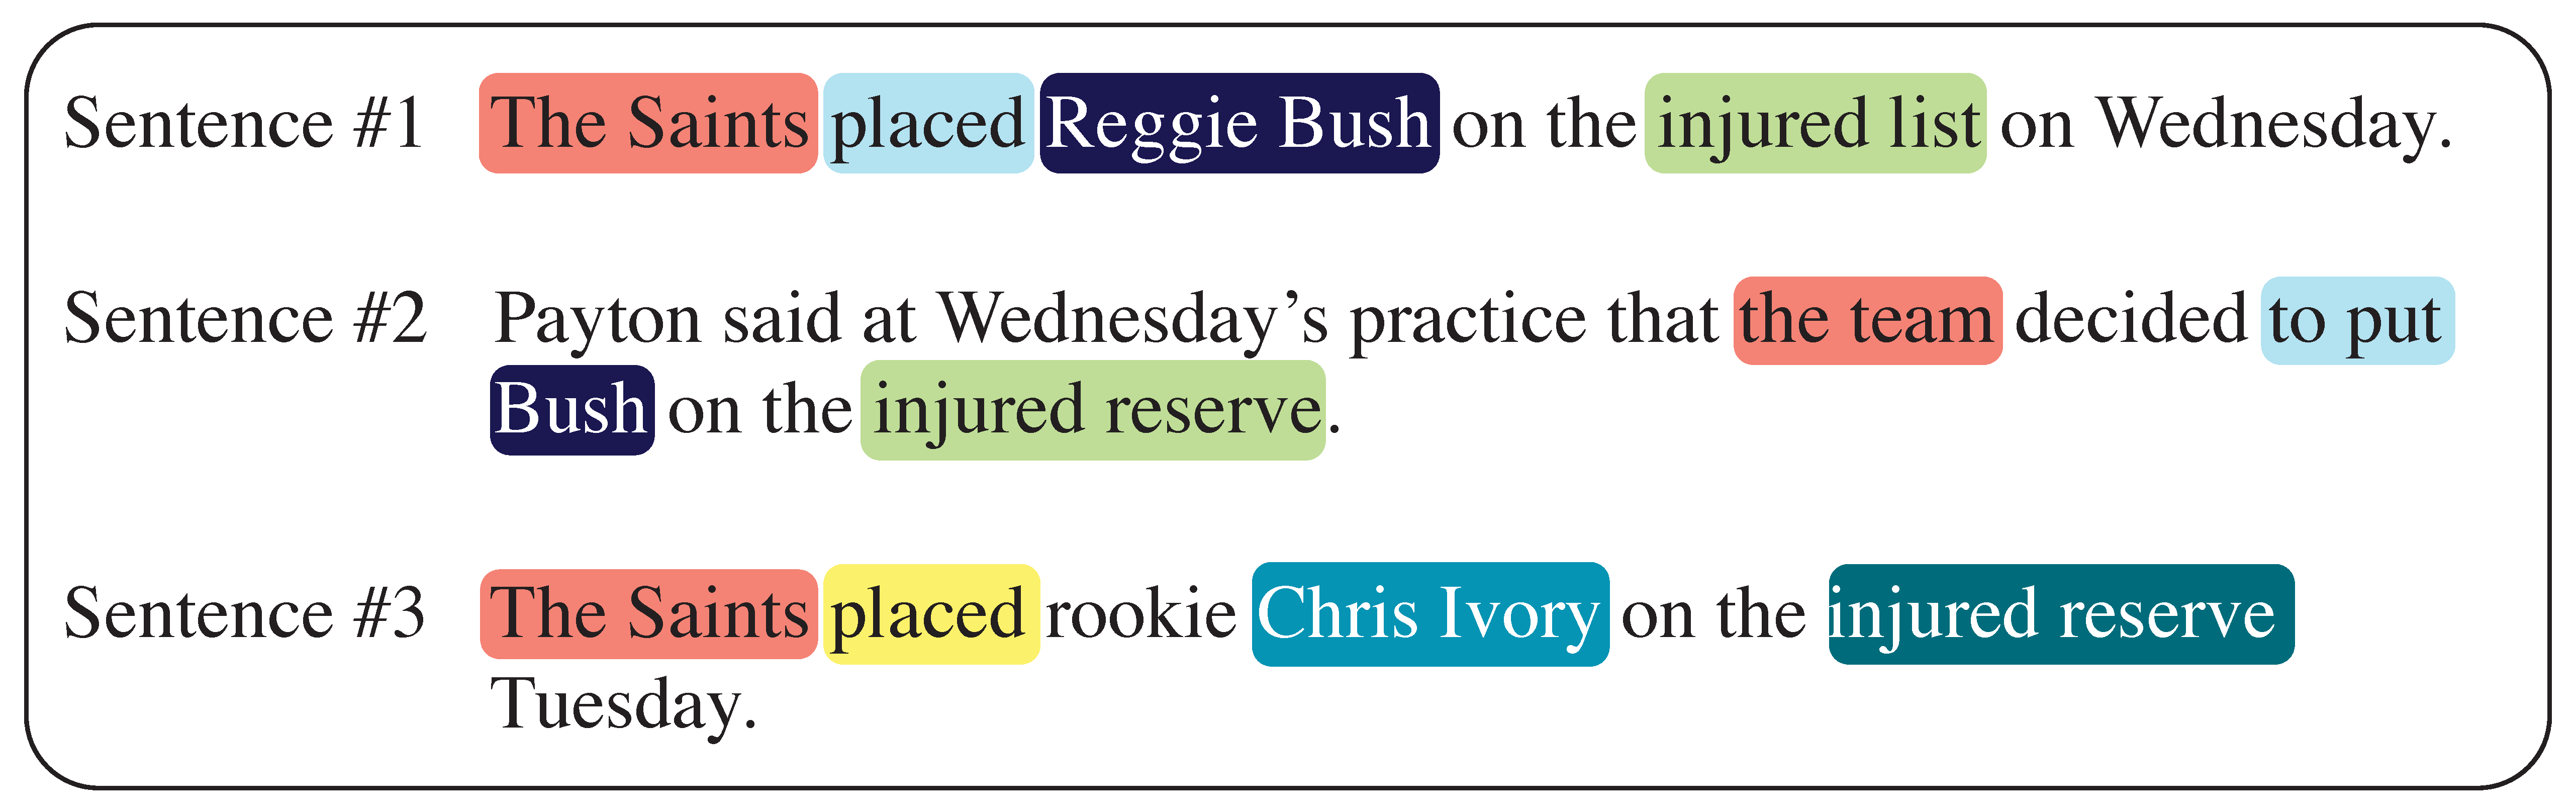
\includegraphics[width=0.65\textwidth]{graphics/corpus}
	\caption{Sample of a coreference resolution corpus (ECB+), depicting gold coref mentions as having shared box colors.}
	\label{fig:corpus}
\end{figure}

Coreference resolution is concerned with linking either entities together and/or events together; that is, entities shall not be linked to events, and doing so would be considered an incorrect link.  Although one may be interested in evaluating coreference systems by their ability to correctly link \textit{pairs} of mentions \cite{parma}, coreference resolution is ultimately a clustering task, whereby we wish to group all like-mentions together, as shown with colored boxes in Figure \ref{fig:corpus}.  Specifically, coreference systems aim to find a globally-optimal fit of mentions to clusters, whereby every mention $m$ in the corpus is assigned to exactly one cluster $C$, such that every ${m_i,m_j} \in C$ are co-referent with each other.  If a given $m_i$ is not anaphoric with any other $m_j$, then it should belong to its own $C$ with a membership of one.

Given a corpus of text documents, coreference resolution can be performed and evaluated on either a \textbf{within-document} or \textbf{cross-document} basis:

\begin{itemize}
\item \textbf{Within-document} is when each mention may only link to either (1) no other mention; or (2) other mentions which are contained in the same document.  Even if the gold truth data denotes a mention should link with a mention from a different document, we ignore these links during the evaluation.
\item \textbf{Cross-document} is when the entire corpus is available for linking; a mention is eligible to be co-referent with mentions in any other document, and the evaluation reflects the same.  As described in \cite{revisit:16}, cross-document evaluation is normally conducted by transforming the entire corpus into a ``meta-document."
\end{itemize}

% ====================
\section{Coreference Systems}
% ====================
Coreference systems are predicated upon first having entity/event mentions identified, via a separate, distinct task called \textit{mention detection}.  Next, these identified mentions are used by coreference resolution models.

\subsection{Mention Detection}
This initial mention identification process is a separate line of research and has remained a fundamental task of NLP for several decades \cite{ner-sekine2007}.  When concerned with entities, research is commonly referred to as \textit{named entity recognition} or \textit{entity recognition}. When concerned with events, research is commonly referred to as \textit{event detection}.

\subsubsection{Named Entity Recognition}
The earliest work started in 1991 with the task of identifying company names \cite{Rau91}.  In 1996, the MUC-6 conference \cite{Grishman:1996:MUC:992628.992709} focused on Information Extraction tasks, which included coining the phrase "named entity" and drastically increasing attention to mention detection.  Early work demonstrated state-of-the-art performance with Hidden Markov Models (HMMs) \cite{Bikel97nymble:a} and Conditional Random Fields (CRFs) \cite{McCallum:2003:ERN:1119176.1119206}.  Presently, the best performing systems use similar models --- but from a deep learning framework --- which include Bi-directional LSTMs \cite{Hochreiter:1997:LSM:1246443.1246450, DBLP:journals/tacl/ChiuN16} and Convolution Neural Nets (CNNs) \cite{ma-hovy:2016:P16-1}.

\subsubsection{Event Detection}
Event Detection has received significantly less attention than Named Entity Recognition; however, the task of semantic role labelling (SRL) addresses a similar and more encompassing problem; SRL is a shallow semantic parsing task, whereby the goal is to identify each predicate in a sentence, along with its constituents and how they fill a semantic role --- specifically, to determine the role (e.g., Agent, Patient, Instrument, etc) and their adjuncts (Locative, Temporal, Manner, etc). \cite{Punyakanok:2008:ISP:1403157.1403162, Gildea:2002:ALS:643092.643093}.  In short, both SRL systems and Event Detection systems have often relied on using many lexical and syntactical features, including those from constituency parsers \cite{Toutanova:2005:JLI:1219840.1219913}, dependency parsers \cite{Johansson:2007:LSS:1621474.1621522}, etc.
However, like entity recognition, recent state-of-the-art systems for Event Detection use Bi-directional LSTMs and CNNs \cite{Feng2016ALN}.

\subsection{Coreference Resolution}
As mentioned, coreference systems aim to create the correct clusters of mentions; however, due to the number of possible mention-to-cluster combinations, finding a globally-optimal assignment of clusters is NP-Hard and thus computationally intractable.  In attempt to avoid this, systems typically perform pairwise-mention predictions, then use those predictions to build clusters. The specific modelling strategies for such approximately fall into two categories: (1) mention-ranking / mention-pairs; and (2) entity-level / event-level, as described below; however, it is worth noting that there is no unanimously-dominate modelling paradigm, as state-of-the-art results often come from any of the ones listed below.

\textbf{Mention-ranking} models define a scoring function $f(m_i,m_j)$ which operates on a mention $m_j$ and possible antecedent $m_i$, where $m_i$ occurs earlier in the document and could be null (represented by $\epsilon$ and denoting that $m_j$ is non-anaphoric); e.g., Wiseman, et. al.'s \cite{DBLP:conf/acl/WisemanRSW15}.  These models aim to find the ideal $m_i$ antecedent for every $m_j$ mention.  After every mention has decided to link to $\epsilon$ or a previous mention, it is common practice to define each cluster simply by joining together all mentions which are connected by a single path.  This is a potential weakness, as it asserts the transitive property holds true (e.g., if $m_3$ predicts $m_2$ as its antecedent, and $m_2$ predicts $m_1$ as its antecedent, then $\{m_1,m2,m3\}$ are all connected, which could be a bad decision, as there is no direct consideration given to the relatedness between $m_1$ and $m_3$.

\textbf{Mention-pair} models score all pairs ($m_i,m_j)$, in contrast to mention-ranking models which aim to find the ideal $m_i$ antecedent for every $m_j$.  After every pair of mentions has been scored, it is common practice to cluster mentions in a best-first or easy-first manner (e.g. agglomerative clustering).  Because mention-pair models base their predictions on the information from just two mentions at a time, they are by definition less expressive than entity/event-level models.  Yet, their inference can be relatively simple and effective, allowing them to be fast and scalable.  Consequently, they have often been the approach used by many state-of-the-art systems \cite{Soon:2001:MLA:972597.972602, DBLP:conf/emnlp/DurrettK13}, including our work described in this proposal.

\textbf{Entity/Event-level} Instead of operating on a mention-level basis, these models differ in that they focus on building a global representation of each underlying entity or event, the basis of which determines each mention's membership \cite{DBLP:conf/naacl/WisemanRS16, clark2016improving}.  These models are attractive due to the intuitive nature of modelling each entity with its own representation; however, challenges include (1) deciding how to represent each entity as it is being developed; (2) decided how many entities to model.

The aim is for the above definitions and descriptions to provide sufficient background to understand all of our subsequent chapters in this proposal, including related research, our research thus far, and our proposed work of (1) combining entity and event coreference into one model; and (2) combining our own in-house mention detection with our coreference models.